\documentclass{standalone}
\usepackage{tikz}
\usetikzlibrary{patterns, positioning}
\usepackage[sfdefault]{ClearSans} %% option 'sfdefault' activates Clear Sans as the default text font
\usepackage[T1]{fontenc}

\begin{document}
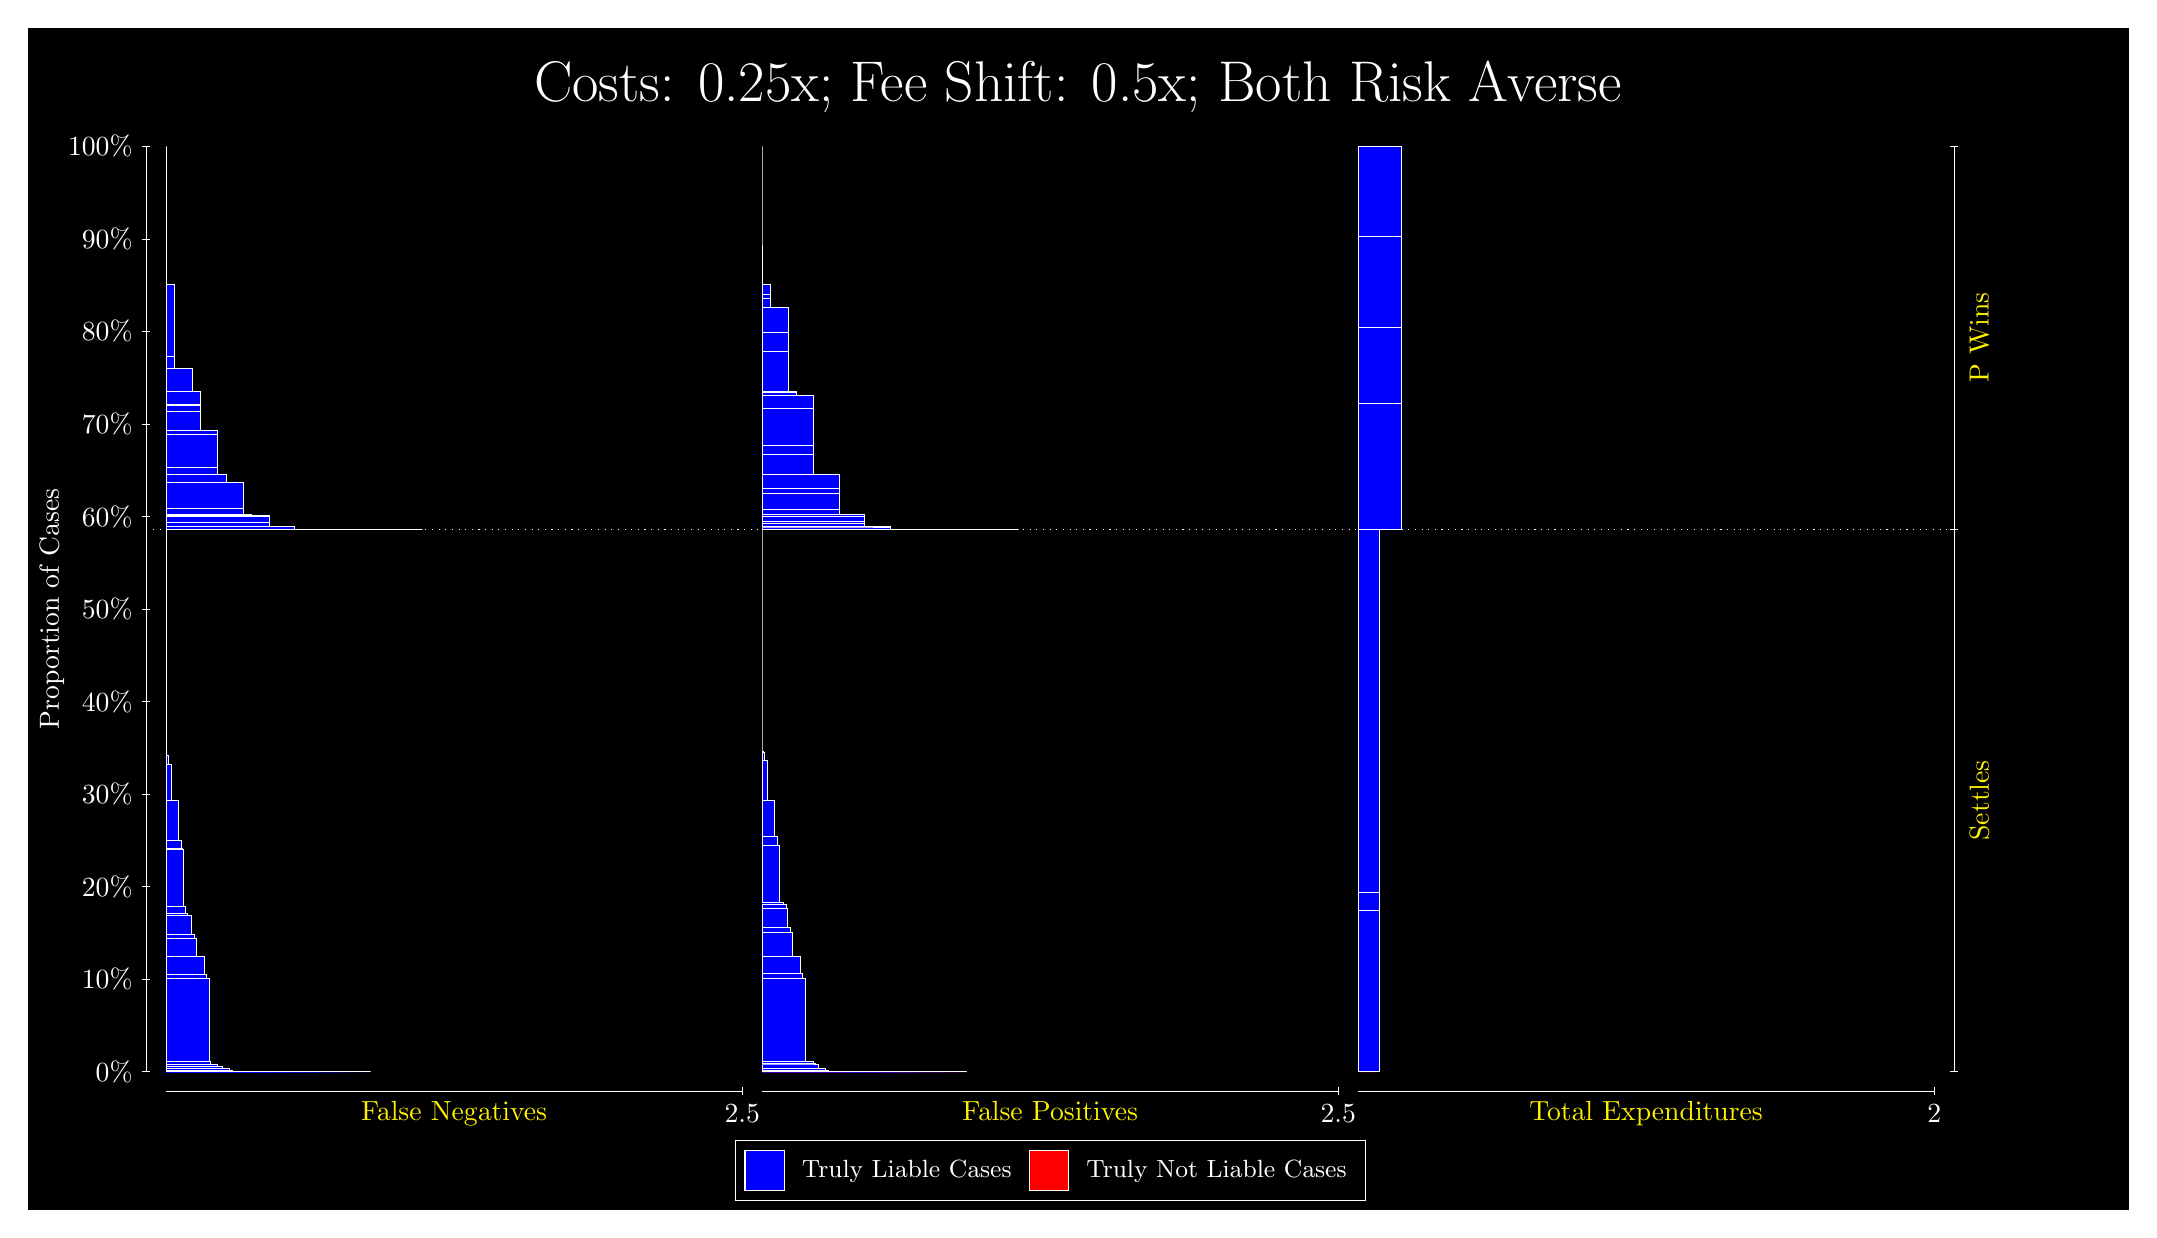
\begin{tikzpicture}
\draw[fill=black] (0,0) rectangle (26.667,15);
\draw[text=white] (0,13.5) rectangle (26.667,15) node[midway] {\huge Costs: 0.25x; Fee Shift: 0.5x; Both Risk Averse};
\draw[white, very thin] (1.5,1.75) -- (1.5,13.5);
\node[rotate=90, text=white, anchor=center] at (0.3, 7.625) {Proportion of Cases};
\draw[white, very thin] (1.45,1.75) -- (1.55,1.75);
\node[text=white, anchor=east] at (1.45, 1.75) {0\%};
\draw[white, very thin] (1.45,2.925) -- (1.55,2.925);
\node[text=white, anchor=east] at (1.45, 2.925) {10\%};
\draw[white, very thin] (1.45,4.1) -- (1.55,4.1);
\node[text=white, anchor=east] at (1.45, 4.1) {20\%};
\draw[white, very thin] (1.45,5.275) -- (1.55,5.275);
\node[text=white, anchor=east] at (1.45, 5.275) {30\%};
\draw[white, very thin] (1.45,6.45) -- (1.55,6.45);
\node[text=white, anchor=east] at (1.45, 6.45) {40\%};
\draw[white, very thin] (1.45,7.625) -- (1.55,7.625);
\node[text=white, anchor=east] at (1.45, 7.625) {50\%};
\draw[white, very thin] (1.45,8.8) -- (1.55,8.8);
\node[text=white, anchor=east] at (1.45, 8.8) {60\%};
\draw[white, very thin] (1.45,9.975) -- (1.55,9.975);
\node[text=white, anchor=east] at (1.45, 9.975) {70\%};
\draw[white, very thin] (1.45,11.15) -- (1.55,11.15);
\node[text=white, anchor=east] at (1.45, 11.15) {80\%};
\draw[white, very thin] (1.45,12.325) -- (1.55,12.325);
\node[text=white, anchor=east] at (1.45, 12.325) {90\%};
\draw[white, very thin] (1.45,13.5) -- (1.55,13.5);
\node[text=white, anchor=east] at (1.45, 13.5) {100\%};

\draw[white, very thin] (24.457,1.75) -- (24.457,13.5);
\draw[white, very thin] (24.407,1.75) -- (24.507,1.75);
\node[anchor=west] at (24.407, 1.75) {};
\draw[white, very thin] (24.407,8.6378) -- (24.507,8.6378);
\node[anchor=west] at (24.407, 8.6378) {};
\draw[white, very thin] (24.407,13.5) -- (24.507,13.5);
\node[anchor=west] at (24.407, 13.5) {};

\draw[white, very thin, fill=blue] (1.75,1.75) rectangle (4.3482,1.75);
\draw[white, very thin, fill=blue] (1.75,1.75) rectangle (4.0554,1.75);
\draw[white, very thin, fill=blue] (1.75,1.75) rectangle (4.0229,1.75);
\draw[white, very thin, fill=blue] (1.75,1.75) rectangle (3.9091,1.75);
\draw[white, very thin, fill=blue] (1.75,1.75) rectangle (3.7627,1.75);
\draw[white, very thin, fill=blue] (1.75,1.75) rectangle (3.7302,1.75);
\draw[white, very thin, fill=blue] (1.75,1.75) rectangle (3.6976,1.75);
\draw[white, very thin, fill=blue] (1.75,1.75) rectangle (3.6163,1.75);
\draw[white, very thin, fill=blue] (1.75,1.75) rectangle (3.5838,1.75);
\draw[white, very thin, fill=blue] (1.75,1.75) rectangle (3.4374,1.75);
\draw[white, very thin, fill=blue] (1.75,1.75) rectangle (3.4049,1.75);
\draw[white, very thin, fill=blue] (1.75,1.75) rectangle (3.3723,1.75);
\draw[white, very thin, fill=blue] (1.75,1.75) rectangle (3.3236,1.75);
\draw[white, very thin, fill=blue] (1.75,1.75) rectangle (3.291,1.75);
\draw[white, very thin, fill=blue] (1.75,1.75) rectangle (3.2585,1.75);
\draw[white, very thin, fill=blue] (1.75,1.75) rectangle (3.1121,1.75);
\draw[white, very thin, fill=blue] (1.75,1.75) rectangle (3.0796,1.75);
\draw[white, very thin, fill=blue] (1.75,1.75) rectangle (3.0471,1.75);
\draw[white, very thin, fill=blue] (1.75,1.75) rectangle (3.0308,1.75);
\draw[white, very thin, fill=blue] (1.75,1.75) rectangle (2.9983,1.75);
\draw[white, very thin, fill=blue] (1.75,1.75) rectangle (2.9657,1.75);
\draw[white, very thin, fill=blue] (1.75,1.75) rectangle (2.9332,1.75);
\draw[white, very thin, fill=blue] (1.75,1.75) rectangle (2.8844,1.751);
\draw[white, very thin, fill=blue] (1.75,1.751) rectangle (2.7868,1.7515);
\draw[white, very thin, fill=blue] (1.75,1.7515) rectangle (2.7543,1.7516);
\draw[white, very thin, fill=blue] (1.75,1.7516) rectangle (2.7218,1.7521);
\draw[white, very thin, fill=blue] (1.75,1.7521) rectangle (2.7055,1.7521);
\draw[white, very thin, fill=blue] (1.75,1.7521) rectangle (2.673,1.7523);
\draw[white, very thin, fill=blue] (1.75,1.7523) rectangle (2.6405,1.754);
\draw[white, very thin, fill=blue] (1.75,1.754) rectangle (2.6079,1.7541);
\draw[white, very thin, fill=blue] (1.75,1.7541) rectangle (2.5917,1.7637);
\draw[white, very thin, fill=blue] (1.75,1.7637) rectangle (2.5591,1.7909);
\draw[white, very thin, fill=blue] (1.75,1.7909) rectangle (2.4616,1.8146);
\draw[white, very thin, fill=blue] (1.75,1.8146) rectangle (2.429,1.8191);
\draw[white, very thin, fill=blue] (1.75,1.8191) rectangle (2.3965,1.8433);
\draw[white, very thin, fill=blue] (1.75,1.8433) rectangle (2.3802,1.8433);
\draw[white, very thin, fill=blue] (1.75,1.8433) rectangle (2.3477,1.8479);
\draw[white, very thin, fill=blue] (1.75,1.8479) rectangle (2.3152,1.8779);
\draw[white, very thin, fill=blue] (1.75,1.8779) rectangle (2.2989,2.9299);
\draw[white, very thin, fill=blue] (1.75,2.9299) rectangle (2.2827,2.9317);
\draw[white, very thin, fill=blue] (1.75,2.9317) rectangle (2.2664,2.988);
\draw[white, very thin, fill=blue] (1.75,2.988) rectangle (2.2339,3.2171);
\draw[white, very thin, fill=blue] (1.75,3.2171) rectangle (2.1363,3.439);
\draw[white, very thin, fill=blue] (1.75,3.439) rectangle (2.1037,3.4879);
\draw[white, very thin, fill=blue] (1.75,3.4879) rectangle (2.0712,3.7344);
\draw[white, very thin, fill=blue] (1.75,3.7344) rectangle (2.055,3.7349);
\draw[white, very thin, fill=blue] (1.75,3.7349) rectangle (2.0224,3.7585);
\draw[white, very thin, fill=blue] (1.75,3.7585) rectangle (1.9899,3.8449);
\draw[white, very thin, fill=blue] (1.75,3.8449) rectangle (1.9736,4.5751);
\draw[white, very thin, fill=blue] (1.75,4.5751) rectangle (1.9574,4.5798);
\draw[white, very thin, fill=blue] (1.75,4.5798) rectangle (1.9411,4.6907);
\draw[white, very thin, fill=blue] (1.75,4.6907) rectangle (1.9086,5.1939);
\draw[white, very thin, fill=blue] (1.75,5.1939) rectangle (1.811,5.6526);
\draw[white, very thin, fill=blue] (1.75,5.6526) rectangle (1.7785,5.7613);
\draw[white, very thin, fill=red] (1.75,5.7613) rectangle (1.75,5.7613);
\draw[white, very thin, fill=blue] (1.75,5.7613) rectangle (1.75,8.6378);
\draw[white, very thin, fill=blue] (1.75,8.6378) rectangle (5.0069,8.6378);
\draw[white, very thin, fill=blue] (1.75,8.6378) rectangle (4.6816,8.6378);
\draw[white, very thin, fill=blue] (1.75,8.6378) rectangle (4.3563,8.6378);
\draw[white, very thin, fill=blue] (1.75,8.6378) rectangle (4.1368,8.6378);
\draw[white, very thin, fill=blue] (1.75,8.6378) rectangle (4.031,8.6379);
\draw[white, very thin, fill=blue] (1.75,8.6379) rectangle (4.031,8.638);
\draw[white, very thin, fill=blue] (1.75,8.638) rectangle (3.8115,8.638);
\draw[white, very thin, fill=blue] (1.75,8.638) rectangle (3.7058,8.6399);
\draw[white, very thin, fill=blue] (1.75,8.6399) rectangle (3.7058,8.6412);
\draw[white, very thin, fill=blue] (1.75,8.6412) rectangle (3.4862,8.6412);
\draw[white, very thin, fill=blue] (1.75,8.6412) rectangle (3.4862,8.6412);
\draw[white, very thin, fill=blue] (1.75,8.6412) rectangle (3.3805,8.6698);
\draw[white, very thin, fill=blue] (1.75,8.6698) rectangle (3.1609,8.6698);
\draw[white, very thin, fill=blue] (1.75,8.6698) rectangle (3.1609,8.6698);
\draw[white, very thin, fill=blue] (1.75,8.6698) rectangle (3.0552,8.7225);
\draw[white, very thin, fill=blue] (1.75,8.7225) rectangle (3.0552,8.7972);
\draw[white, very thin, fill=blue] (1.75,8.7972) rectangle (3.0552,8.8132);
\draw[white, very thin, fill=blue] (1.75,8.8132) rectangle (2.8356,8.8205);
\draw[white, very thin, fill=blue] (1.75,8.8205) rectangle (2.8356,8.8205);
\draw[white, very thin, fill=blue] (1.75,8.8205) rectangle (2.8356,8.8209);
\draw[white, very thin, fill=blue] (1.75,8.8209) rectangle (2.7299,8.9069);
\draw[white, very thin, fill=blue] (1.75,8.9069) rectangle (2.7299,9.2356);
\draw[white, very thin, fill=blue] (1.75,9.2356) rectangle (2.5103,9.2364);
\draw[white, very thin, fill=blue] (1.75,9.2364) rectangle (2.5103,9.3304);
\draw[white, very thin, fill=blue] (1.75,9.3304) rectangle (2.4046,9.424);
\draw[white, very thin, fill=blue] (1.75,9.424) rectangle (2.4046,9.8463);
\draw[white, very thin, fill=blue] (1.75,9.8463) rectangle (2.4046,9.8945);
\draw[white, very thin, fill=blue] (1.75,9.8945) rectangle (2.1851,10.134);
\draw[white, very thin, fill=blue] (1.75,10.134) rectangle (2.1851,10.206);
\draw[white, very thin, fill=blue] (1.75,10.206) rectangle (2.1851,10.222);
\draw[white, very thin, fill=blue] (1.75,10.222) rectangle (2.1851,10.39);
\draw[white, very thin, fill=blue] (1.75,10.39) rectangle (2.0793,10.678);
\draw[white, very thin, fill=blue] (1.75,10.678) rectangle (1.8598,10.833);
\draw[white, very thin, fill=blue] (1.75,10.833) rectangle (1.8598,11.748);
\draw[white, very thin, fill=blue] (1.75,11.748) rectangle (1.7541,11.796);
\draw[white, very thin, fill=blue] (1.75,11.796) rectangle (1.7541,11.796);
\draw[white, very thin, fill=red] (1.75,11.796) rectangle (1.75,11.796);
\draw[white, very thin, fill=blue] (1.75,11.796) rectangle (1.75,13.5);
\draw[white, very thin, fill=red] (9.3189,1.75) rectangle (11.917,1.75);
\draw[white, very thin, fill=blue] (9.3189,1.75) rectangle (11.917,1.75);
\draw[white, very thin, fill=red] (9.3189,1.75) rectangle (11.624,1.75);
\draw[white, very thin, fill=blue] (9.3189,1.75) rectangle (11.624,1.75);
\draw[white, very thin, fill=blue] (9.3189,1.75) rectangle (11.592,1.75);
\draw[white, very thin, fill=red] (9.3189,1.75) rectangle (11.332,1.75);
\draw[white, very thin, fill=blue] (9.3189,1.75) rectangle (11.332,1.75);
\draw[white, very thin, fill=blue] (9.3189,1.75) rectangle (11.299,1.75);
\draw[white, very thin, fill=blue] (9.3189,1.75) rectangle (11.266,1.75);
\draw[white, very thin, fill=red] (9.3189,1.75) rectangle (11.185,1.75);
\draw[white, very thin, fill=blue] (9.3189,1.75) rectangle (11.185,1.75);
\draw[white, very thin, fill=blue] (9.3189,1.75) rectangle (11.006,1.75);
\draw[white, very thin, fill=blue] (9.3189,1.75) rectangle (10.974,1.75);
\draw[white, very thin, fill=blue] (9.3189,1.75) rectangle (10.941,1.75);
\draw[white, very thin, fill=red] (9.3189,1.75) rectangle (10.892,1.75);
\draw[white, very thin, fill=blue] (9.3189,1.75) rectangle (10.892,1.75);
\draw[white, very thin, fill=blue] (9.3189,1.75) rectangle (10.86,1.75);
\draw[white, very thin, fill=blue] (9.3189,1.75) rectangle (10.681,1.75);
\draw[white, very thin, fill=blue] (9.3189,1.75) rectangle (10.648,1.75);
\draw[white, very thin, fill=blue] (9.3189,1.75) rectangle (10.616,1.75);
\draw[white, very thin, fill=red] (9.3189,1.75) rectangle (10.6,1.75);
\draw[white, very thin, fill=blue] (9.3189,1.75) rectangle (10.6,1.75);
\draw[white, very thin, fill=blue] (9.3189,1.75) rectangle (10.567,1.75);
\draw[white, very thin, fill=blue] (9.3189,1.75) rectangle (10.535,1.75);
\draw[white, very thin, fill=red] (9.3189,1.75) rectangle (10.453,1.75);
\draw[white, very thin, fill=blue] (9.3189,1.75) rectangle (10.453,1.751);
\draw[white, very thin, fill=blue] (9.3189,1.751) rectangle (10.356,1.7533);
\draw[white, very thin, fill=blue] (9.3189,1.7533) rectangle (10.323,1.7535);
\draw[white, very thin, fill=red] (9.3189,1.7535) rectangle (10.307,1.7535);
\draw[white, very thin, fill=blue] (9.3189,1.7535) rectangle (10.307,1.7535);
\draw[white, very thin, fill=blue] (9.3189,1.7535) rectangle (10.291,1.754);
\draw[white, very thin, fill=blue] (9.3189,1.754) rectangle (10.274,1.7541);
\draw[white, very thin, fill=blue] (9.3189,1.7541) rectangle (10.242,1.7542);
\draw[white, very thin, fill=blue] (9.3189,1.7542) rectangle (10.209,1.7542);
\draw[white, very thin, fill=red] (9.3189,1.7542) rectangle (10.161,1.7542);
\draw[white, very thin, fill=blue] (9.3189,1.7542) rectangle (10.161,1.7638);
\draw[white, very thin, fill=blue] (9.3189,1.7638) rectangle (10.128,1.7909);
\draw[white, very thin, fill=blue] (9.3189,1.7909) rectangle (10.03,1.8445);
\draw[white, very thin, fill=blue] (9.3189,1.8445) rectangle (9.9979,1.8508);
\draw[white, very thin, fill=blue] (9.3189,1.8508) rectangle (9.9816,1.851);
\draw[white, very thin, fill=blue] (9.3189,1.851) rectangle (9.9654,1.8752);
\draw[white, very thin, fill=blue] (9.3189,1.8752) rectangle (9.9491,1.8797);
\draw[white, very thin, fill=blue] (9.3189,1.8797) rectangle (9.9166,1.8842);
\draw[white, very thin, fill=blue] (9.3189,1.8842) rectangle (9.884,1.8843);
\draw[white, very thin, fill=red] (9.3189,1.8843) rectangle (9.8678,1.8843);
\draw[white, very thin, fill=blue] (9.3189,1.8843) rectangle (9.8678,2.9363);
\draw[white, very thin, fill=blue] (9.3189,2.9363) rectangle (9.8353,2.9924);
\draw[white, very thin, fill=blue] (9.3189,2.9924) rectangle (9.8027,3.2171);
\draw[white, very thin, fill=blue] (9.3189,3.2171) rectangle (9.7051,3.5248);
\draw[white, very thin, fill=blue] (9.3189,3.5248) rectangle (9.6726,3.5784);
\draw[white, very thin, fill=blue] (9.3189,3.5784) rectangle (9.6563,3.5806);
\draw[white, very thin, fill=blue] (9.3189,3.5806) rectangle (9.6401,3.8271);
\draw[white, very thin, fill=blue] (9.3189,3.8271) rectangle (9.6238,3.8721);
\draw[white, very thin, fill=blue] (9.3189,3.8721) rectangle (9.5913,3.8957);
\draw[white, very thin, fill=blue] (9.3189,3.8957) rectangle (9.5588,3.8962);
\draw[white, very thin, fill=blue] (9.3189,3.8962) rectangle (9.5425,4.6264);
\draw[white, very thin, fill=blue] (9.3189,4.6264) rectangle (9.51,4.7352);
\draw[white, very thin, fill=blue] (9.3189,4.7352) rectangle (9.4774,5.1939);
\draw[white, very thin, fill=blue] (9.3189,5.1939) rectangle (9.3799,5.697);
\draw[white, very thin, fill=blue] (9.3189,5.697) rectangle (9.3473,5.8079);
\draw[white, very thin, fill=blue] (9.3189,5.8079) rectangle (9.3311,5.8127);
\draw[white, very thin, fill=blue] (9.3189,5.8127) rectangle (9.3189,8.6378);
\draw[white, very thin, fill=red] (9.3189,8.6378) rectangle (12.576,8.6378);
\draw[white, very thin, fill=blue] (9.3189,8.6378) rectangle (12.576,8.6378);
\draw[white, very thin, fill=red] (9.3189,8.6378) rectangle (12.25,8.6378);
\draw[white, very thin, fill=blue] (9.3189,8.6378) rectangle (12.25,8.6378);
\draw[white, very thin, fill=blue] (9.3189,8.6378) rectangle (11.925,8.6378);
\draw[white, very thin, fill=red] (9.3189,8.6378) rectangle (11.925,8.6378);
\draw[white, very thin, fill=blue] (9.3189,8.6378) rectangle (11.925,8.6378);
\draw[white, very thin, fill=blue] (9.3189,8.6378) rectangle (11.6,8.6378);
\draw[white, very thin, fill=blue] (9.3189,8.6378) rectangle (11.6,8.6379);
\draw[white, very thin, fill=red] (9.3189,8.6379) rectangle (11.6,8.6379);
\draw[white, very thin, fill=blue] (9.3189,8.6379) rectangle (11.6,8.638);
\draw[white, very thin, fill=red] (9.3189,8.638) rectangle (11.275,8.638);
\draw[white, very thin, fill=blue] (9.3189,8.638) rectangle (11.275,8.6399);
\draw[white, very thin, fill=blue] (9.3189,8.6399) rectangle (11.275,8.6406);
\draw[white, very thin, fill=blue] (9.3189,8.6406) rectangle (11.275,8.6412);
\draw[white, very thin, fill=red] (9.3189,8.6412) rectangle (11.055,8.6412);
\draw[white, very thin, fill=blue] (9.3189,8.6412) rectangle (11.055,8.6412);
\draw[white, very thin, fill=red] (9.3189,8.6412) rectangle (10.949,8.6412);
\draw[white, very thin, fill=blue] (9.3189,8.6412) rectangle (10.949,8.6646);
\draw[white, very thin, fill=blue] (9.3189,8.6646) rectangle (10.949,8.6698);
\draw[white, very thin, fill=blue] (9.3189,8.6698) rectangle (10.73,8.6698);
\draw[white, very thin, fill=red] (9.3189,8.6698) rectangle (10.73,8.6698);
\draw[white, very thin, fill=blue] (9.3189,8.6698) rectangle (10.73,8.6698);
\draw[white, very thin, fill=blue] (9.3189,8.6698) rectangle (10.624,8.7158);
\draw[white, very thin, fill=blue] (9.3189,8.7158) rectangle (10.624,8.7321);
\draw[white, very thin, fill=red] (9.3189,8.7321) rectangle (10.624,8.7321);
\draw[white, very thin, fill=blue] (9.3189,8.7321) rectangle (10.624,8.7984);
\draw[white, very thin, fill=blue] (9.3189,8.7984) rectangle (10.624,8.8209);
\draw[white, very thin, fill=blue] (9.3189,8.8209) rectangle (10.404,8.8209);
\draw[white, very thin, fill=red] (9.3189,8.8209) rectangle (10.404,8.8209);
\draw[white, very thin, fill=blue] (9.3189,8.8209) rectangle (10.404,8.8209);
\draw[white, very thin, fill=blue] (9.3189,8.8209) rectangle (10.299,8.8866);
\draw[white, very thin, fill=blue] (9.3189,8.8866) rectangle (10.299,9.0892);
\draw[white, very thin, fill=red] (9.3189,9.0892) rectangle (10.299,9.0892);
\draw[white, very thin, fill=blue] (9.3189,9.0892) rectangle (10.299,9.1565);
\draw[white, very thin, fill=blue] (9.3189,9.1565) rectangle (10.299,9.3302);
\draw[white, very thin, fill=blue] (9.3189,9.3302) rectangle (10.079,9.3302);
\draw[white, very thin, fill=red] (9.3189,9.3302) rectangle (10.079,9.3302);
\draw[white, very thin, fill=blue] (9.3189,9.3302) rectangle (10.079,9.3304);
\draw[white, very thin, fill=blue] (9.3189,9.3304) rectangle (9.9735,9.5859);
\draw[white, very thin, fill=blue] (9.3189,9.5859) rectangle (9.9735,9.7062);
\draw[white, very thin, fill=blue] (9.3189,9.7062) rectangle (9.9735,10.176);
\draw[white, very thin, fill=blue] (9.3189,10.176) rectangle (9.9735,10.342);
\draw[white, very thin, fill=blue] (9.3189,10.342) rectangle (9.7539,10.342);
\draw[white, very thin, fill=red] (9.3189,10.342) rectangle (9.7539,10.342);
\draw[white, very thin, fill=blue] (9.3189,10.342) rectangle (9.7539,10.379);
\draw[white, very thin, fill=blue] (9.3189,10.379) rectangle (9.7539,10.39);
\draw[white, very thin, fill=blue] (9.3189,10.39) rectangle (9.6482,10.9);
\draw[white, very thin, fill=blue] (9.3189,10.9) rectangle (9.6482,11.144);
\draw[white, very thin, fill=blue] (9.3189,11.144) rectangle (9.6482,11.46);
\draw[white, very thin, fill=blue] (9.3189,11.46) rectangle (9.4287,11.572);
\draw[white, very thin, fill=red] (9.3189,11.572) rectangle (9.4287,11.572);
\draw[white, very thin, fill=blue] (9.3189,11.572) rectangle (9.4287,11.618);
\draw[white, very thin, fill=blue] (9.3189,11.618) rectangle (9.4287,11.748);
\draw[white, very thin, fill=blue] (9.3189,11.748) rectangle (9.3229,11.825);
\draw[white, very thin, fill=blue] (9.3189,11.825) rectangle (9.3229,12.113);
\draw[white, very thin, fill=blue] (9.3189,12.113) rectangle (9.3229,12.243);
\draw[white, very thin, fill=blue] (9.3189,12.243) rectangle (9.3189,13.5);
\draw[white, very thin, fill=red] (16.888,1.75) rectangle (17.162,1.75);
\draw[white, very thin, fill=blue] (16.888,1.75) rectangle (17.162,3.8032);
\draw[white, very thin, fill=red] (16.888,3.8032) rectangle (17.162,3.8032);
\draw[white, very thin, fill=blue] (16.888,3.8032) rectangle (17.162,4.0311);
\draw[white, very thin, fill=red] (16.888,4.0311) rectangle (17.162,4.0311);
\draw[white, very thin, fill=blue] (16.888,4.0311) rectangle (17.162,8.6378);
\draw[white, very thin, fill=red] (16.888,8.6378) rectangle (17.437,8.6378);
\draw[white, very thin, fill=blue] (16.888,8.6378) rectangle (17.437,10.239);
\draw[white, very thin, fill=red] (16.888,10.239) rectangle (17.437,10.239);
\draw[white, very thin, fill=blue] (16.888,10.239) rectangle (17.437,11.203);
\draw[white, very thin, fill=red] (16.888,11.203) rectangle (17.437,11.203);
\draw[white, very thin, fill=blue] (16.888,11.203) rectangle (17.437,12.361);
\draw[white, very thin, fill=red] (16.888,12.361) rectangle (17.437,12.361);
\draw[white, very thin, fill=blue] (16.888,12.361) rectangle (17.437,13.5);
\draw[white, dotted] (1.5,8.6378) -- (24.457,8.6378);
\draw[white, very thin] (1.75,1.5) -- (9.0689,1.5);
\node[text=yellow, anchor=north] at (5.4094, 1.5) {False Negatives};
\draw[white, very thin] (9.0689,1.45) -- (9.0689,1.55);
\node[text=white, anchor=north] at (9.0689, 1.45) {2.5};

\draw[white, very thin] (9.3189,1.5) -- (16.638,1.5);
\node[text=yellow, anchor=north] at (12.978, 1.5) {False Positives};
\draw[white, very thin] (16.638,1.45) -- (16.638,1.55);
\node[text=white, anchor=north] at (16.638, 1.45) {2.5};

\draw[white, very thin] (16.888,1.5) -- (24.207,1.5);
\node[text=yellow, anchor=north] at (20.547, 1.5) {Total Expenditures};
\draw[white, very thin] (24.207,1.45) -- (24.207,1.55);
\node[text=white, anchor=north] at (24.207, 1.45) {2};

\node[text=yellow, centered, rotate=90] at (24.777, 5.1939) {Settles};
\node[text=yellow, centered, rotate=90] at (24.777, 11.069) {P Wins};

\draw (12.978300999999998,1.5) node[draw=none] (baseCoordinate) {};
\begin{scope}[align=center]
        \matrix[scale=0.5, draw=white, below=0.5cm of baseCoordinate, nodes={draw}, column sep=0.1cm]{
            \node[rectangle, draw, minimum width=0.5cm, minimum height=0.5cm, fill=blue] {}; &
            \node[draw=none, font=\small, text=white] (B) {Truly Liable Cases}; &
            \node[rectangle, draw, minimum width=0.5cm, minimum height=0.5cm, fill=red] {}; &
            \node[draw=none, font=\small, text=white] (B) {Truly Not Liable Cases}; \\
            };
\end{scope}

\end{tikzpicture}
\end{document}